% !TeX root = ../../Skript.tex
\cohead{\Large\textbf{Fläche zwischen 2 Funktionen}}
\fakesubsection{Fläche zwischen Zwei Funktionen}
\begin{tcolorbox}
	\textbf{Fläche zwischen 2 Funktionen \(f(x)\) und \(g(x)\):}

	\textcolor{loestc}{Das folgende Integral bestimmt die orientierte Fläche zwischen den beiden Funktionen:
		\[\int_a^b f(x)-g(x) \td x\]
		Dabei ist der Wert des Integrals positiv, falls \(f(x)>g(x)\) (Das Schaubild von \(f(x)\) liegt oberhalb des Schaubilds von \(g(x)\)). Liegt das Schaubild von \(g(x)\) oberhalb von \(f(x)\), ist der Wert des Integrals negativ.
	}
\end{tcolorbox}
\begin{minipage}{\textwidth}
	\adjustbox{valign=t}{\begin{minipage}{.6\textwidth}\raggedright
		Beispiele:\\
		Bestimme den Flächeninhalt, der zwischen \textcolor{blue}{\(f(x)=x+1\)} und \textcolor{red}{\(g(x)=0,5x^2-3\)} eingeschlossenen Fläche.\\
		\textcolor{loes}{Die Integrationsgrenzen ergeben sich aus den Schnittstellen der beiden Funktionen:}
		\textcolor{loes}{Aus \(f(x)=g(x)\) ergibt sich mit Hilfe der Mitternachtsformel \(x_1=-2,\ x_2=4\)}.\\
		\textcolor{loes}{Da die Gerade \(f(x)\) im relevanten Bereich oberhalb der Parabel \(g(x)\) liegt, muss man über \(f(x)-g(x)\) integrieren:}
		\begin{align*}
			\textcolor{loes}{\int_{-2}^4 f(x)-g(x) \td x}&\textcolor{loes}{\;=\int_{-2}^4 x+1-\left(0,5x^2-3\right) \td x}\\
			&\textcolor{loes}{\;=\left[-\tfrac{1}{6}x^3+\tfrac{1}{2}x^2+4x\right]_{-2}^4=18}
		\end{align*}
	\end{minipage}}%
	\adjustbox{valign=t, padding=3ex 0ex 0ex 0ex}{\begin{minipage}{.4\textwidth-3ex}
		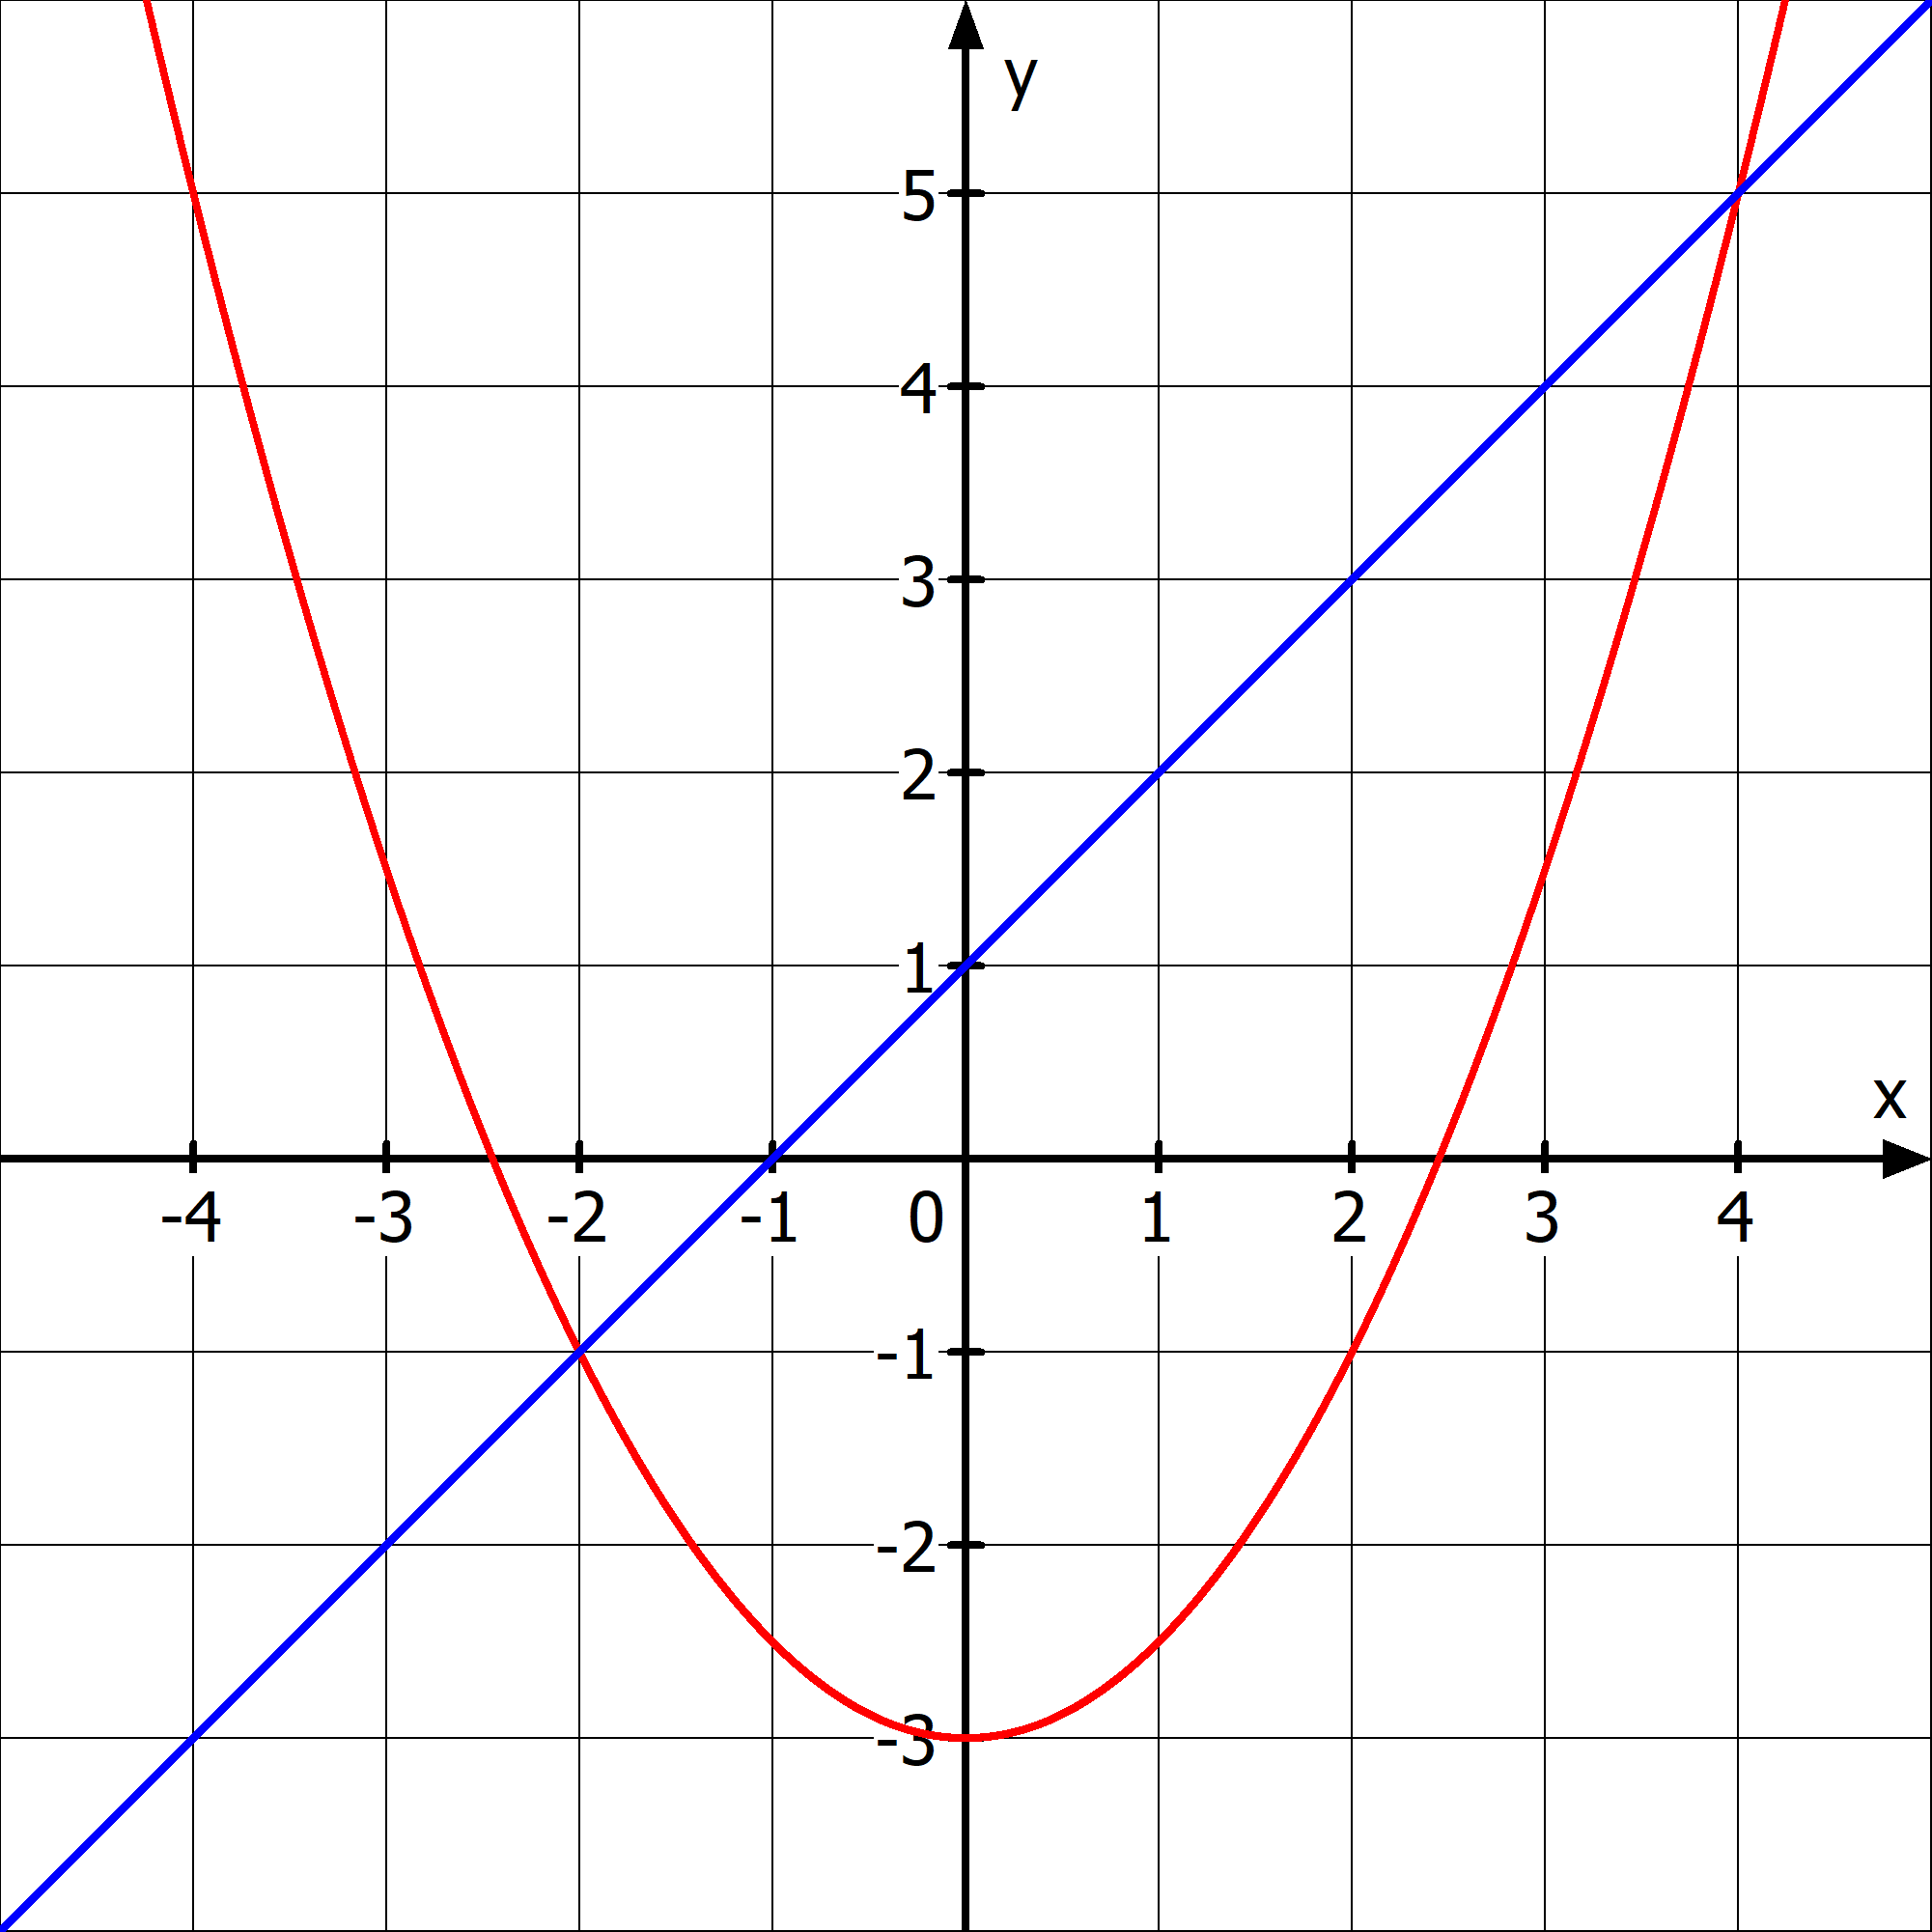
\includegraphics[width=\linewidth]{\integration/pics/FlaecheZwZweiFktBsp.png}
	\end{minipage}}%
\end{minipage}

\vspace{2cm}

\begin{minipage}{\textwidth}
	\adjustbox{valign=t, padding=0ex 0ex 3ex 0ex}{\begin{minipage}{.4\textwidth-3ex}
		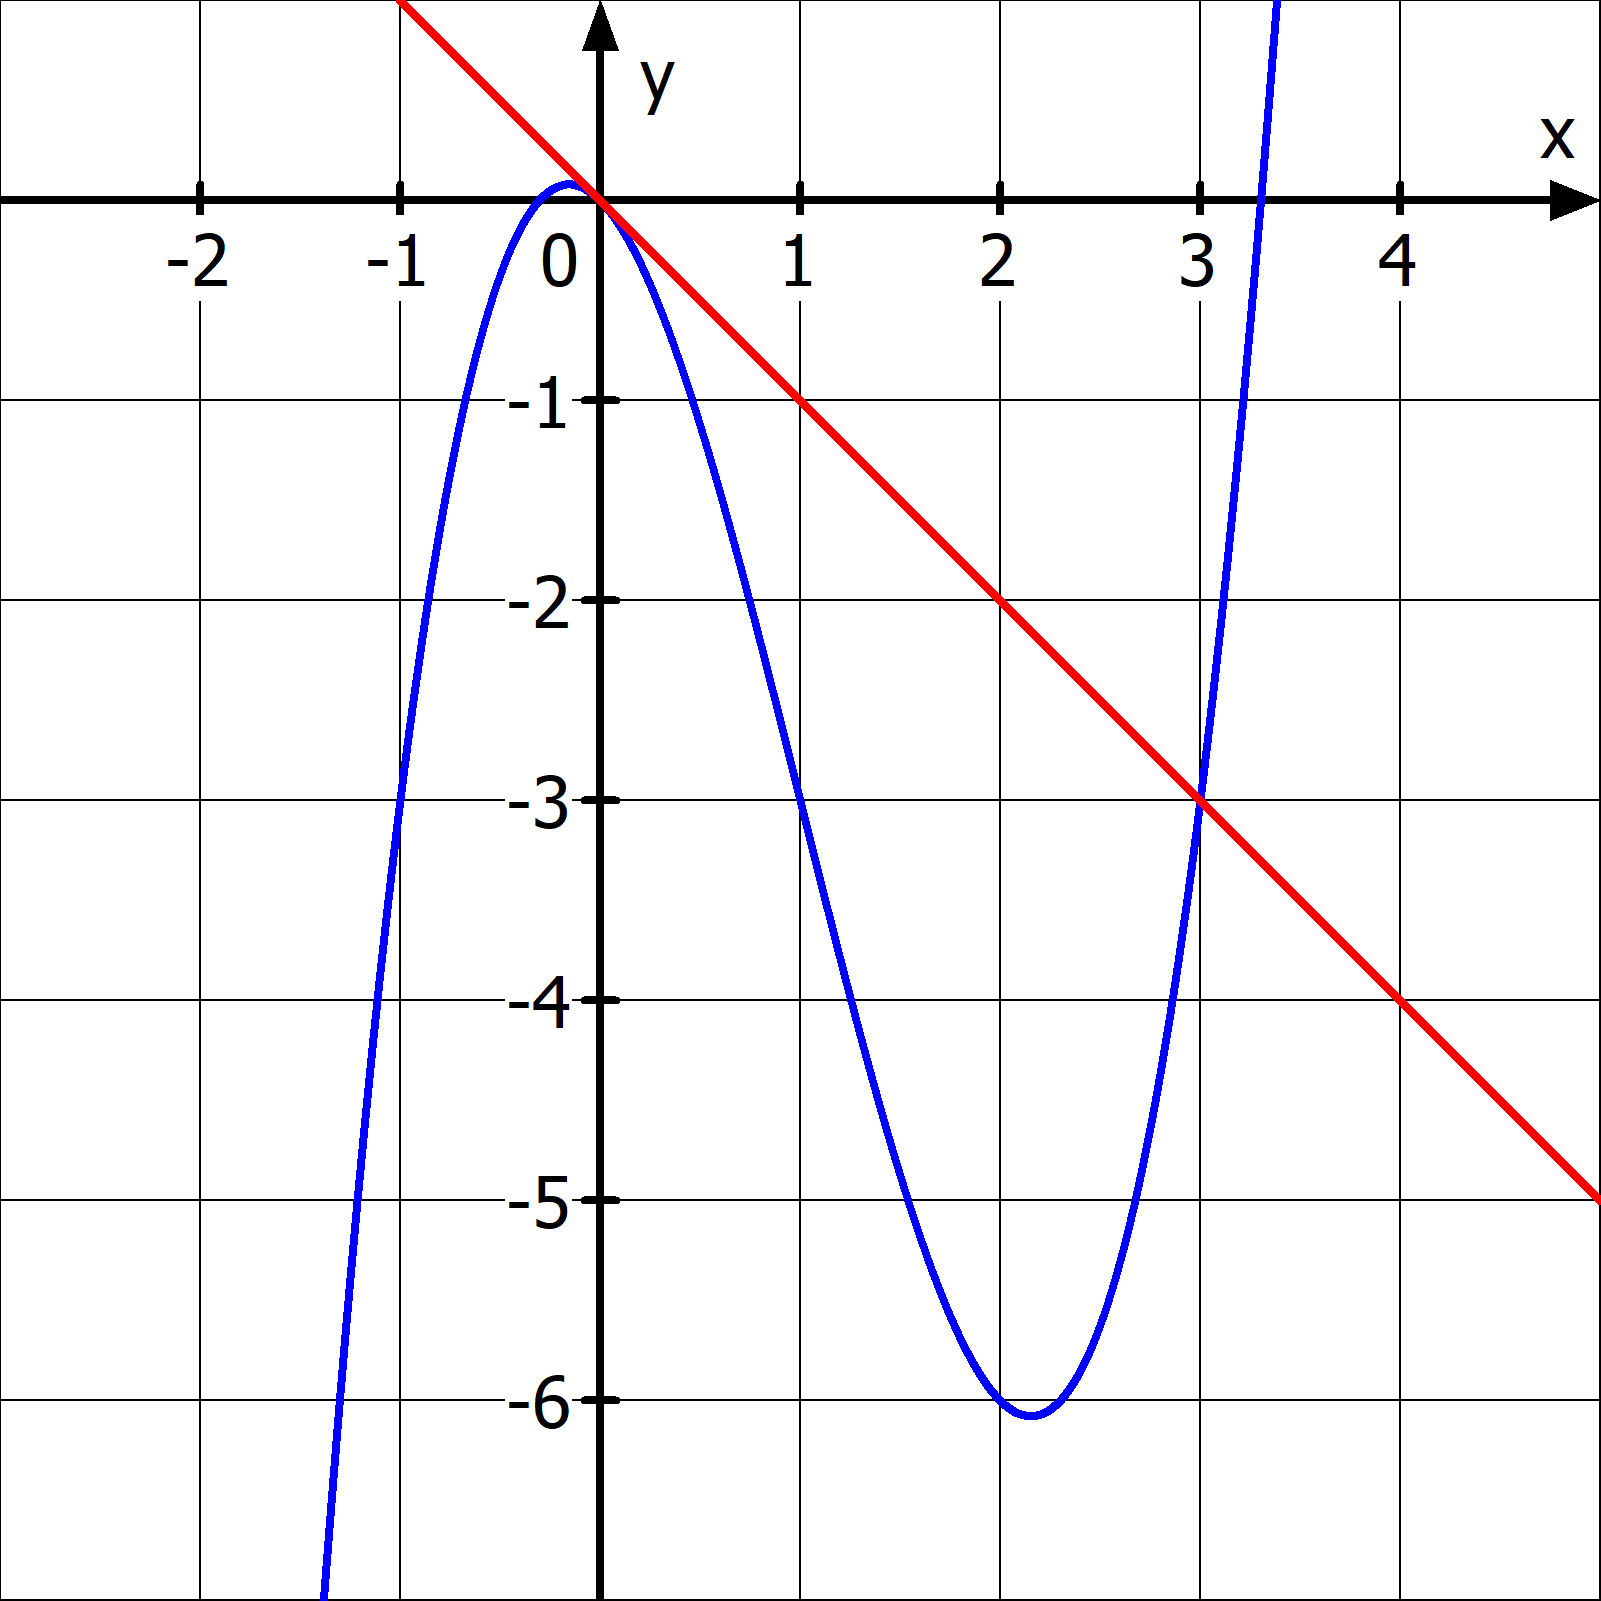
\includegraphics[width=\linewidth]{\integration/pics/FlaecheZwZweiFktBsp2.png}
	\end{minipage}}%
	\adjustbox{valign=t}{\begin{minipage}{.6\textwidth}\raggedright
		Bestimme den Flächeninhalt, der zwischen \textcolor{blue}{\(f(x)=x^3-3x^2-x\)} und \textcolor{red}{\(g(x)=-x\)} eingeschlossenen Fläche.\\
		\textcolor{loes}{Die Integrationsgrenzen ergeben sich aus den Schnittstellen der beiden Funktionen:}
		\textcolor{loes}{Aus \(f(x)=g(x)\) ergibt sich \(x_1=0,\ x_2=3\)}.\\
		\textcolor{loes}{Da die Gerade \(g(x)\) im relevanten Bereich oberhalb der ganzrationalen Funktion \(f(x)\) liegt, muss man über \(g(x)-f(x)\) integrieren:}
		\begin{align*}
			\textcolor{loes}{\int_{0}^3 g(x)-f(x) \td x}&\textcolor{loes}{\;=\int_{0}^3 -x-\left(x^3-3x^2-x\right) \td x}\\
			&\textcolor{loes}{\;=\int_{0}^3 -x^3+3x^2 \td x}\\
			&\textcolor{loes}{\;=\left[-\tfrac{1}{4}x^4+x^3\right]_{0}^3=6,75}
		\end{align*}
	\end{minipage}}%
\end{minipage}
\newpage

\begin{Exercise}[title={\raggedright\normalfont Bestimme jeweils die zwischen den beiden Funktionen eingeschlossene Fläche.}, label=flaecheZwFkt1]
	\begin{enumerate}[label=\alph*)]
		\item \(f(x)=-2x\) und \(g(x)=x^2-x-2\)
		\item \(f(x)=-\frac{1}{4}x^2+4\) und \(g(x)=-x+1\)
		\item \(f(x)=3\) und \(g(x)=x^3-2x^2-3x+3\)
		\item \(f(x)=2x^2-12x+15\) und \(g(x)=-x^2+6x-9\)
		\item \(f(x)=\frac{1}{2}x^2-4x-1\) und \(g(x)=-2x-1\)
		\item \(f(x)=-2x+2\) und \(g(x)=\frac{1}{4}x^3-\frac{1}{4}x^2-\frac{7}{2}x+2\)
	\end{enumerate}
\end{Exercise}

%%%%%%%%%%%%%%%%%%%%%%%%%%%%%%%%%%%%%%%%%
\begin{Answer}[ref=flaecheZwFkt1]
	\begin{enumerate}[label=\alph*)]
		\item \(\displaystyle\int_{-2}^1 -2x-\left(x^2-x-2\right) \td x=4,5\)
		\item \(\displaystyle\int_{-2}^{6} -\frac{1}{4}x^2+4-\left(-x+1\right) \td x=\frac{64}{3}\)
		\item \(\displaystyle\int_{-1}^{0} x^3-2x^2-3x+3-\left(3\right) \td x+\int_{0}^{3} 3-\left(x^3-2x^2-3x+3\right) \td x=\frac{7}{12}+\frac{45}{4}=\frac{71}{6}\)
		\item \(\displaystyle\int_{2}^{4} -x^2+6x-9-\left(2x^2-12x+15\right) \td x=4\)
		\item \(\displaystyle\int_{0}^{4} -2x-1-\left(\frac{1}{2}x^2-4x-1\right) \td x=\frac{16}{3}\)
		\item \(\displaystyle\int_{-2}^{0} \frac{1}{4}x^3-\frac{1}{4}x^2-\frac{7}{2}x+2-\left(-2x+2\right) \td x+\int_{0}^{3} -2x+2-\left(\frac{1}{4}x^3-\frac{1}{4}x^2-\frac{7}{2}x+2\right) \td x=\frac{4}{3}+\frac{63}{16}=\frac{253}{48}\)
	\end{enumerate}
\end{Answer}